\documentclass[a4paper]{article}
\usepackage[utf8x]{inputenc}
\usepackage[T1,T2A]{fontenc}
\usepackage[russian]{babel}
\usepackage{hyperref}
\usepackage{indentfirst}
\usepackage{listings}
\usepackage{color}
\usepackage{here}
\usepackage{array}
\usepackage{multirow}
\usepackage{graphicx}
\usepackage{multicol}

\usepackage{caption}
\renewcommand{\lstlistingname}{Программа} % заголовок листингов кода

\usepackage{listings}
\lstset{ %
extendedchars=\true,
keepspaces=true,
language=bash,					% choose the language of the code
basicstyle=\footnotesize,		% the size of the fonts that are used for the code
numbers=left,					% where to put the line-numbers
numberstyle=\footnotesize,		% the size of the fonts that are used for the line-numbers
stepnumber=1,					% the step between two line-numbers. If it is 1 each line will be numbered
numbersep=5pt,					% how far the line-numbers are from the code
backgroundcolor=\color{white},	% choose the background color. You must add \usepackage{color}
showspaces=false				% show spaces adding particular underscores
showstringspaces=false,			% underline spaces within strings
showtabs=false,					% show tabs within strings adding particular underscores
frame=single,           		% adds a frame around the code
tabsize=2,						% sets default tabsize to 2 spaces
captionpos=b,					% sets the caption-position to bottom
breaklines=true,				% sets automatic line breaking
breakatwhitespace=false,		% sets if automatic breaks should only happen at whitespace
escapeinside={\%*}{*)},			% if you want to add a comment within your code
postbreak=\raisebox{0ex}[0ex][0ex]{\ensuremath{\color{red}\hookrightarrow\space}}
}

\lstdefinestyle{customc}{
  belowcaptionskip=1\baselineskip,
  breaklines=true,
  frame=L,
  xleftmargin=\parindent,
  language=C,
  showstringspaces=false,
  basicstyle=\footnotesize\ttfamily,
  keywordstyle=\bfseries\color{green!40!black},
  commentstyle=\itshape\color{purple!40!black},
  identifierstyle=\color{blue},
  stringstyle=\color{orange},
}

\usepackage[left=2cm,right=2cm,
top=2cm,bottom=2cm,bindingoffset=0cm]{geometry}


\begin{document}	% начало документа

\begin{titlepage}	% начало титульной страницы

	\begin{center}		% выравнивание по центру

		\large Санкт-Петербургский политехнический университет Петра Великого\\
		\large Институт компьютерных наук и технологий \\
		\large Кафедра компьютерных систем и программных технологий\\[6cm]
		% название института, затем отступ 6см
		
		\huge Отчет по курсовой работе\\[0.5cm] % название работы, затем отступ 0,5см
		\large по дисциплине <<Параллельные вычисления>>\\[0.1cm]
		\large тема работы: <<Определение площади набора кругов, заданных массивом с координатами центров и радиусами, методом Монте-Карло.>>\\[0.1cm]

	\end{center}


	\begin{flushright} % выравнивание по правому краю
		\begin{minipage}{0.25\textwidth} % врезка в половину ширины текста
			\begin{flushleft} % выровнять её содержимое по левому краю

				\large\textbf{Работу выполнил:}\\
				\large Косолапов С.А.\\
				\large {Группа:} 53501/3\\
				
				\large \textbf{Преподаватель:}\\
				\large Стручков И.В.

			\end{flushleft}
		\end{minipage}
	\end{flushright}
	
	\vfill % заполнить всё доступное ниже пространство

	\begin{center}
	\large Санкт-Петербург\\
	\large \the\year % вывести дату
	\end{center} % закончить выравнивание по центру

\thispagestyle{empty} % не нумеровать страницу
\end{titlepage} % конец титульной страницы

\vfill % заполнить всё доступное ниже пространство



% Содержание
\tableofcontents
\newpage


\section{Постановка задачи}

\begin{enumerate}
\item Реализовать последовательную программу, позволяющую определить суммарную площадь набора кругов, заданных массивом с координатами центров и радиусами, методом Монте-Карло. 

\item Провести тестирование последовательной программы.

\item Реализовать параллельные программы с использованием PThreads и MPI.

\item Провести тестирование производительности параллельных программ в зависимости от количества используемых ядер (процессоров).

\item Проанализировать полученные результаты и сделать выводы.
\end{enumerate}

\section{Реализация}

Поставленная задача была декомпозирована на следующие этапы:

\begin{enumerate}

\item Загрузка координат центра круга и его радиуса из файла. Результатом является контейнер объектов, содержащих координаты и радиус кругов.

\item Определение площади с использованием метода Монте-Карло. Определяются граничные точки заданных кругов, образующие прямоугольную область. В соответствии с заданной плотностью случайным образом сгенерированных точек внутри прямоугольной области, а также её площадью, устанавливается их количество. Каждая точка проверяется на принадлежность хотя бы одному из кругов. Таким образом, предельное отношение точек, принадлежащих хотя бы одному из кругов, к общему количеству сгенерированных точек, примерно равняется суммарной площади кругов.

\item Вывод результата и статистических показателей, таких как математическое ожидание результата и его дисперсия.

\end{enumerate}

\subsection{Реализация последовательной программы}

В соответствии с решаемыми задачами, исходный код программы содержит в себе следующие файлы:

\begin{enumerate}

\item types.h - содержит структуры и переопределённые типы, используемые в программе

\lstinputlisting[language=C++, firstline=10, lastline=89]{../CirclesFigureArea/types.h}

В файле содержатся структуры Point, Circle и Rect, а также определён тип RandomFunction, позволяющий использовать различные варианты генерации точек.

\item parser.h и parser.cpp - содержат в себе объявление и реализацию функции, позволяющей считать вектор объектов типа Circle из файла

\lstinputlisting[language=C++, firstline=35, lastline=35]{../CirclesFigureArea/parser.h}

\item solver.h и solver.cpp - содержат функциональность для решения задачи

\lstinputlisting[language=C++, firstline=19, lastline=23]{../CirclesFigureArea/solver.h}

Функция solve позволяет решить задачу для кругов, указанных в параметре circles. Также указываются параметры density - количество точек на единицу площади (плотность генерации) и random - функция для генерации точек со случайными координатами. Сама функция solve вызывает функцию getFigureRect, которая позволяет определить границы прямоугольной области, в которой находятся круги, а затем - функцию generateAndCheckPoints, возвращающую общее количество точек и количество точек, входящих в круги.

Функция getFigureRect:

\lstinputlisting[language=C++, firstline=47, lastline=81]{../CirclesFigureArea/solver.cpp}

В функции generateAndCheckPoints производится непосредственное решение задачи. Изначально определяется количество точек для генерации:

\lstinputlisting[language=C++, firstline=23, lastline=25]{../CirclesFigureArea/solver.cpp}

Затем с помощью функции генерации random, передаваемой как параметр функции, генерируются точки и проверяются на принадлежность кругам.

\lstinputlisting[language=C++, firstline=31, lastline=38]{../CirclesFigureArea/solver.cpp}

Функция isPointInsideCircles позволяет проверить, находится ли точка внутри окружностей:

\lstinputlisting[language=C++, firstline=84, lastline=94]{../CirclesFigureArea/solver.cpp}

\item randomizer.h и randomizer.cpp - содержат функции для генерации точек со случайными координатами.

Рассмотрено два варианта реализации функций генерации точек.

\begin{enumerate}
	\item random\_simple - позволяет решить задачу с помощью функции rand() и последующего масштабирования на заданную прямоугольную область. У данной реализации имеются две основные проблемы - распределение отлично от равномерного, что создаёт дополнительную погрешность, а также невозможность одновременного использования функции несколькими потоками, что затрудняет использование данной функции при работе с PThreads и OpenMP.
			
	\item random\_uniform\_real\_distribution - позволяет решить задачу с использованием функции,  генерирующей равномерное распределение (std::uniform\_real\_distribution). Этот вариант хорошо работает в параллельных приложениях, а также позволяет получить действительно равномерное распределение. Основной проблемой является достаточно медленное выполнение функции.
	
\end{enumerate}

Таким образом, после первоначального тестирования и выявления недостатков функции random\_simple было решено вдальнейшем использовать random\_uniform\_real\_distribution.

\item main.cpp соединяет воедино функциональность программы, содержит тесты.

\end{enumerate}

\subsection{Реализация параллельной программы с использованием PThreads}

В данном случае дополнительно создаются N-1 потоков, если считать N количеством ядер. Количество генерируемых точек COUNT делится на N частей, и созданные потоки генерируют и проверяют принадлежность окружностям для COUNT/N точек. Оставшиеся COUNT - (N-1)*COUNT/N точек генерируются и проверяются главным потоком. Затем главный поток выполняет pthread\_join для всех созданных потоков и, когда дождётся, может сложить полученные всеми потоками результаты. Результаты хранятся в массиве, адрес элементов которого передаётся каждому потоку.

Так как в pthread\_create тип передаваемых параметров void*, в функцию передаётся указатель на следующую структуру, позволяющую потоку использовать необходимые значения:


\lstinputlisting[language=C++, firstline=92, lastline=112]{../CirclesFigureAreaPosix/types.h}

Функция, реализующая функциональность одного потока:

\lstinputlisting[language=C++, firstline=20, lastline=33]{../CirclesFigureAreaPosix/solver.cpp}

Таким образом, для каждого потока генерируется и проверяется на принадлежность кругам заданное количество точек.

В функции generateAndCheckPoints сначала создаются потоки:

\lstinputlisting[language=C++, firstline=52, lastline=64]{../CirclesFigureAreaPosix/solver.cpp}

Затем производятся вычисления на главном потоке:

\lstinputlisting[language=C++, firstline=66, lastline=69]{../CirclesFigureAreaPosix/solver.cpp}

После этого главный поток ожидает созданные потоки, либо удостоверяется в их завершении:

\lstinputlisting[language=C++, firstline=71, lastline=74]{../CirclesFigureAreaPosix/solver.cpp}

Сделав это, главный поток проводит редукцию результатов:

\lstinputlisting[language=C++, firstline=78, lastline=84]{../CirclesFigureAreaPosix/solver.cpp}

Полученное значение делится на общее количество точек, и получается суммарная площадь, занимаемая кругами.

В данном случае удалось избежать совместного использования потоками ресурсов для записи, а следовательно, и использования средств синхронизации.

\subsection{Реализация параллельной программы с использованием MPI}

В данном случае создаются не потоки, а процессы. Запуск программы в этом случае должен осуществляться с помощью программы mpirun. Использована реализация OpenMPI.

Это создаёт дополнительные шаги и при использовании MPI в программе. В частности, необходимо произвести инициализацию и финализацию с помощью функций MPI\_Init и MPI\_Finalize. Причём в MPI\_Init необходимо также передать аргументы командной строки, поэтому её использование вне функции main затруднено в связи с необходимостью передачи дополнительных параметров.

MPI использует понятия группы и коммуникатора. Группа процессов - это упорядоченная коллекция процессов. Коммуникатор же позволяет общаться процессам внутри группы или между группами.

Также в программе используется функция MPI\_Comm\_size, позволяющая получить размер коммуникатора, а также стандартный коммуникатор MPI\_COMM\_WORLD, содержащий все созданные процессы.

С помощью функции MPI\_Comm\_rank можно узнать номер процесса в текущем коммуникаторе.

Функция generateAndCheckPoints видоизменилась, и теперь её часть, решающая задачу, выглядит следующим образом:

\lstinputlisting[language=C++, firstline=58, lastline=86]{../CirclesFigureAreaMPI/solver.cpp}

Таким образом, в зависимости от ранга процесса, мы определяем, главный это процесс или нет. Он должен ожидать результат от остальных процессов и выполнить редукцию.

Передача и получение результата выделены в отдельные функции:

\lstinputlisting[language=C++, firstline=36, lastline=45]{../CirclesFigureAreaMPI/solver.cpp}

Используется блокирующая передача сообщений, при которой процесс-отправитель ожидает, пока процесс-получатель примет переданное сообщение.

Непосредственное решение задачи также вынесено в отдельную функцию:

\lstinputlisting[language=C++, firstline=20, lastline=34]{../CirclesFigureAreaMPI/solver.cpp}


\section{Тестирование производительности многозадачных программ}

Для обеих многозадачных модификаций программ были проведены тестовые испытания, состоящие из 50 тестов для различного количества ядер от 1 до 6.


\subsection{Многопоточная программа с использованием POSIX Threads}

Результат, в зависимости от количества задействованных потоков:

\begin{itemize}
	\item 1 поток
		\lstinputlisting[firstline=258, lastline=264]{../CirclesFigureAreaPosix/results.log}
	\item 2 потока
		\lstinputlisting[firstline=519, lastline=525]{../CirclesFigureAreaPosix/results.log}
	\item 3 потока
		\lstinputlisting[firstline=780, lastline=786]{../CirclesFigureAreaPosix/results.log}
	\item 4 потока
		\lstinputlisting[firstline=1041, lastline=1047]{../CirclesFigureAreaPosix/results.log}
	\item 5 потоков
		\lstinputlisting[firstline=1302, lastline=1308]{../CirclesFigureAreaPosix/results.log}
	\item 6 потоков
		\lstinputlisting[firstline=1563, lastline=1569]{../CirclesFigureAreaPosix/results.log}
\end{itemize}

\begin{figure}[H]
	\begin{center}
		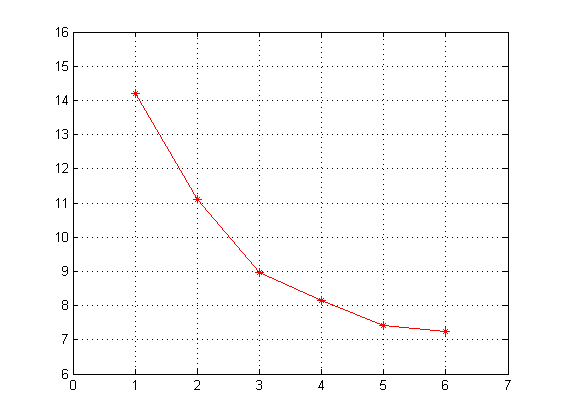
\includegraphics[scale=0.7]{pic/posix.png}
		\caption{График зависимости времени выполнения программы с PThreads от количества ядер} 
		\label{pic:pic_name} % название для ссылок внутри кода
	\end{center}
\end{figure}

В данном случае с увеличением количества ядер наблюдается лишь незначительное увеличение производительности. Так, при использовании 6 ядер программа выполняется быстрее всего в 2 раза.

\subsection{Многопроцессная программа с использованием MPI}

Тестирование программы осуществляется с помощью shell-скрипта runtest.sh:

\lstinputlisting[language=sh]{../CirclesFigureAreaMPI/runtest.sh}

Результат, в зависимости от количества задействованных процессов:

\begin{itemize}
	\item 1 процесс
		\lstinputlisting[firstline=159, lastline=165]{../CirclesFigureAreaMPI/results.log}
	\item 2 процесса
		\lstinputlisting[firstline=376, lastline=382]{../CirclesFigureAreaMPI/results.log}
	\item 3 процесса
		\lstinputlisting[firstline=644, lastline=650]{../CirclesFigureAreaMPI/results.log}
	\item 4 процесса
		\lstinputlisting[firstline=962, lastline=968]{../CirclesFigureAreaMPI/results.log}
	\item 5 процессов
		\lstinputlisting[firstline=1330, lastline=1336]{../CirclesFigureAreaMPI/results.log}
	\item 6 процессов
		\lstinputlisting[firstline=1747, lastline=1753]{../CirclesFigureAreaMPI/results.log}
\end{itemize}

\begin{figure}[H]
	\begin{center}
		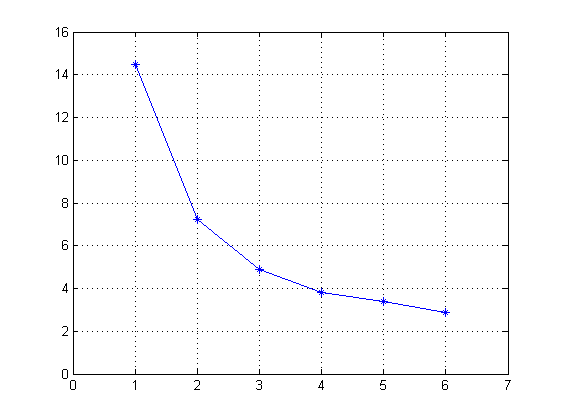
\includegraphics[scale=0.7]{pic/mpi.png}
		\caption{График зависимости времени выполнения программы с MPI от количества ядер} 
		\label{pic:pic_name} % название для ссылок внутри кода
	\end{center}
\end{figure}

Как видно из графика и листингов, в данном случае наблюдается существенное ускорение выполнения программы. На 6 ядрах, в сравнении с одним, программа выполняется на 80\% быстрее, т.е. достигается ускорение в 5 раз, по сравнению с программой, использующей одно ядро.


\section{Выводы}

В работе исследованы варианты преобразования последовательной программы в параллельную с использованием технологий POSIX Threads и MPI. PThreads позволяют использовать параллельно несколько потоков. Главным достоиноством такого подхода является отсутствие разделения адресных пространств взаимодействующих задач, что  избавляет от необходимости задумываться о межпроцессном взаимодействии, а также позволяет локализовать изменения программы в случае преобразования её реализации из последовательной в параллельную. Вместе с тем, данный способ дал не очень большое повышение производительности. Скорее всего, это связано с использованием функции генерации случайных значений, обращение к которой невозможно произвести параллельно для одного процесса.

Технология MPI, наоборот, позволила реализовать приложение, производительность которого существенно улучшается с увеличением числа ядер, на которых оно исполняется. Межпроцессное взаимодействие внутри данной технологии осуществляется путём передачи сообщений между задачами и удобно при использовании простых типов передаваемых данных. Вместе с тем, чтобы передать сложные структуры данных между процессами, их придётся декомпозировать до простых типов, которые можно использовать в функциях MPI\_Send и MPI\_Recv. Определённым недостатком технологии можно считать необходимость изменения функции main с целью вставки туда MPI\_Init и MPI\_Finalize. В остальном изменения, связанные с распараллеливанием программы с использованием MPI локальны.


\section{Листинги}

Файлы parser.h, parser.cpp, randomizer.h и randomizer.cpp являются общими для всех программ. Файлы main.cpp, types.h, solver.h и solver.cpp изменены, в соответствии с реализациями.

\begin{enumerate}
\item Последовательная программа
	\begin{itemize}
		\item main.cpp
			\lstinputlisting[language=C++]{../CirclesFigureArea/main.cpp}
		\item types.h
			\lstinputlisting[language=C++]{../CirclesFigureArea/types.h}
		\item parse.h
			\lstinputlisting[language=C++]{../CirclesFigureArea/parser.h}
		\item parse.cpp
			\lstinputlisting[language=C++]{../CirclesFigureArea/parser.cpp}
		\item solve.h
			\lstinputlisting[language=C++]{../CirclesFigureArea/solver.h}
		\item solve.cpp
			\lstinputlisting[language=C++]{../CirclesFigureArea/solver.cpp}
		\item randomize.h
			\lstinputlisting[language=C++]{../CirclesFigureArea/randomizer.h}
		\item randomize.cpp
			\lstinputlisting[language=C++]{../CirclesFigureArea/randomizer.cpp}
	\end{itemize}
	
\item Модифицированная с использованием PThreads программа
	\begin{itemize}
		\item main.cpp
			\lstinputlisting[language=C++]{../CirclesFigureAreaPosix/main.cpp}
		\item types.h
			\lstinputlisting[language=C++]{../CirclesFigureAreaPosix/types.h}
		\item solve.h
			\lstinputlisting[language=C++]{../CirclesFigureAreaPosix/solver.h}
		\item solve.cpp
			\lstinputlisting[language=C++]{../CirclesFigureAreaPosix/solver.cpp}
	\end{itemize}
	
\item Модифицированная с использованием MPI программа
	\begin{itemize}
		\item main.cpp
			\lstinputlisting[language=C++]{../CirclesFigureAreaMPI/main.cpp}
		\item types.h
			\lstinputlisting[language=C++]{../CirclesFigureAreaMPI/types.h}
		\item solve.h
			\lstinputlisting[language=C++]{../CirclesFigureAreaMPI/solver.h}
		\item solve.cpp
			\lstinputlisting[language=C++]{../CirclesFigureAreaMPI/solver.cpp}
	\end{itemize}
\end{enumerate}

\end{document}